\section{Peta Karnaugh 4 Variabel}

Peta Karnaugh 4 variabel merupakan bentuk K-Map yang paling umum digunakan dalam praktik perancangan rangkaian digital. Peta ini terdiri dari $2^4 = 16$ sel yang disusun dalam grid $4 \times 4$, dengan dua variabel pada sumbu baris dan dua variabel pada sumbu kolom, keduanya mengikuti urutan Kode Gray. Pada konfigurasi ini, properti wrap-around berlaku pada kedua sumbu: kolom pertama bersebelahan dengan kolom terakhir, dan baris pertama bersebelahan dengan baris terakhir \cite{rosen2019}.

\subsection{Struktur K-Map 4 Variabel}

Gambar~\ref{fig:kmap-4var} menampilkan struktur K-Map 4 variabel dengan variabel $A, B$ pada baris dan $C, D$ pada kolom. Setiap sel berisi notasi minterm $m_j$ yang berkorespondensi dengan kombinasi input biner.

\begin{figure}[htbp]
\centering
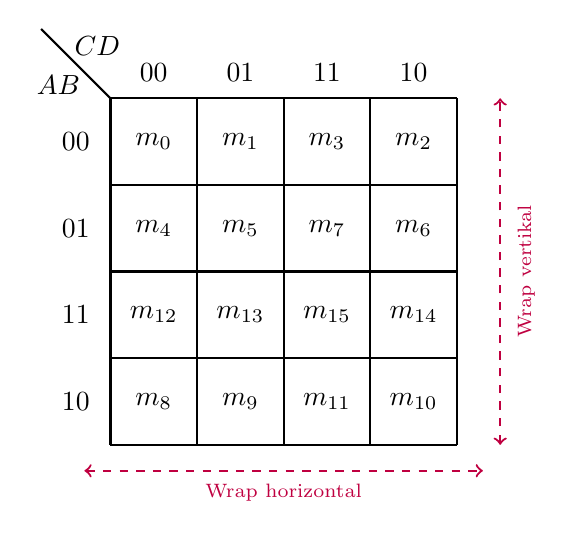
\begin{tikzpicture}[scale=1.1]
    % Grid 4x4
    \draw[thick] (0,0) grid (4,4);
    % Diagonal divider
    \draw[thick] (0,4) -- (-0.8,4.8);
    \node at (-0.6, 4.15) {$AB$};
    \node at (-0.15, 4.6) {$CD$};
    % Labels x-axis (Gray)
    \node at (0.5, 4.3) {$00$}; \node at (1.5, 4.3) {$01$}; \node at (2.5, 4.3) {$11$}; \node at (3.5, 4.3) {$10$};
    % Labels y-axis (Gray)
    \node at (-0.4, 3.5) {$00$}; \node at (-0.4, 2.5) {$01$}; \node at (-0.4, 1.5) {$11$}; \node at (-0.4, 0.5) {$10$};
    % Cells row 00
    \node at (0.5, 3.5) {$m_0$}; \node at (1.5, 3.5) {$m_1$}; \node at (2.5, 3.5) {$m_3$}; \node at (3.5, 3.5) {$m_2$};
    % Cells row 01
    \node at (0.5, 2.5) {$m_4$}; \node at (1.5, 2.5) {$m_5$}; \node at (2.5, 2.5) {$m_7$}; \node at (3.5, 2.5) {$m_6$};
    % Cells row 11
    \node at (0.5, 1.5) {$m_{12}$}; \node at (1.5, 1.5) {$m_{13}$}; \node at (2.5, 1.5) {$m_{15}$}; \node at (3.5, 1.5) {$m_{14}$};
    % Cells row 10
    \node at (0.5, 0.5) {$m_8$}; \node at (1.5, 0.5) {$m_9$}; \node at (2.5, 0.5) {$m_{11}$}; \node at (3.5, 0.5) {$m_{10}$};
    % Wrap-around indicators
    \draw[<->, thick, purple, dashed] (-0.3, -0.3) -- (4.3, -0.3);
    \node[purple, font=\scriptsize] at (2, -0.55) {Wrap horizontal};
    \draw[<->, thick, purple, dashed] (4.5, 0) -- (4.5, 4);
    \node[purple, font=\scriptsize, rotate=90] at (4.8, 2) {Wrap vertikal};
\end{tikzpicture}
\caption{Struktur Peta Karnaugh 4 Variabel}
\label{fig:kmap-4var}
\end{figure}

Pada K-Map 4 variabel, terdapat beberapa pola kedekatan yang perlu diperhatikan. Selain kedekatan horizontal dan vertikal yang sudah jelas, kedekatan wrap-around terjadi antara kolom $00$ dan $10$ (bersebelahan secara siklis melalui tepi kiri-kanan), serta antara baris $00$ dan $10$ (bersebelahan melalui tepi atas-bawah). Bahkan, keempat sel di empat sudut peta ($m_0, m_2, m_8, m_{10}$) juga secara logis bersebelahan satu sama lain dan dapat membentuk kelompok yang valid.

\subsection{Pola Pengelompokan pada K-Map 4 Variabel}

Pada K-Map 4 variabel, kelompok dapat berukuran 1, 2, 4, 8, atau 16 sel. Tabel berikut merangkum hubungan antara ukuran kelompok dan jumlah variabel yang dieliminasi:

\begin{center}
\renewcommand{\arraystretch}{1.2}
\begin{tabular}{|c|c|l|}
\hline
\textbf{Ukuran} & \textbf{Variabel Dieliminasi} & \textbf{Contoh Suku Hasil} \\ \hline
1 & 0 & $A'B'C'D'$ (minterm lengkap) \\ \hline
2 & 1 & $A'B'C'$ (3 literal) \\ \hline
4 & 2 & $A'B'$ atau $C'D$ (2 literal) \\ \hline
8 & 3 & $A'$ atau $D$ (1 literal) \\ \hline
16 & 4 & $1$ (tautologi) \\ \hline
\end{tabular}
\end{center}

Beberapa pola kelompok khusus yang sering muncul pada K-Map 4 variabel meliputi: (1) kelompok persegi $2 \times 2$ di tengah atau sudut, (2) kelompok satu baris penuh ($1 \times 4$), (3) kelompok satu kolom penuh ($4 \times 1$), dan (4) kelompok ``sudut'' yang mencakup keempat sel di empat pojok peta melalui double wrap-around.

\subsection{Contoh Penyederhanaan K-Map 4 Variabel}

\begin{contoh}
\textbf{Penyederhanaan $F(A,B,C,D) = \sum m(0, 1, 2, 4, 5, 6, 8, 9, 12, 13, 14)$}

\textbf{Langkah 1:} Tempatkan nilai 1 pada K-Map:

\begin{center}
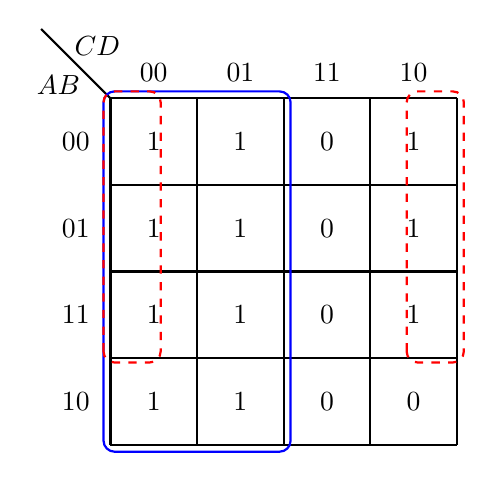
\begin{tikzpicture}[scale=1.1]
    \draw[thick] (0,0) grid (4,4);
    \draw[thick] (0,4) -- (-0.8,4.8);
    \node at (-0.6, 4.15) {$AB$};
    \node at (-0.15, 4.6) {$CD$};
    \node at (0.5, 4.3) {$00$}; \node at (1.5, 4.3) {$01$}; \node at (2.5, 4.3) {$11$}; \node at (3.5, 4.3) {$10$};
    \node at (-0.4, 3.5) {$00$}; \node at (-0.4, 2.5) {$01$}; \node at (-0.4, 1.5) {$11$}; \node at (-0.4, 0.5) {$10$};
    % Values
    \node at (0.5, 3.5) {1}; \node at (1.5, 3.5) {1}; \node at (2.5, 3.5) {0}; \node at (3.5, 3.5) {1};
    \node at (0.5, 2.5) {1}; \node at (1.5, 2.5) {1}; \node at (2.5, 2.5) {0}; \node at (3.5, 2.5) {1};
    \node at (0.5, 1.5) {1}; \node at (1.5, 1.5) {1}; \node at (2.5, 1.5) {0}; \node at (3.5, 1.5) {1};
    \node at (0.5, 0.5) {1}; \node at (1.5, 0.5) {1}; \node at (2.5, 0.5) {0}; \node at (3.5, 0.5) {0};
    % Group 1: left 2 columns (8 cells)
    \draw[thick, blue, rounded corners] (-0.08, -0.08) rectangle (2.08, 4.08);
    % Group 2: right column wrap with left column, rows 00,01,11
    \draw[thick, red, rounded corners, dashed] (3.42, 0.95) rectangle (4.08, 4.08);
    \draw[thick, red, rounded corners, dashed] (-0.08, 0.95) rectangle (0.58, 4.08);
\end{tikzpicture}
\end{center}

\textbf{Langkah 2:} Identifikasi kelompok:
\begin{itemize}
    \item \textcolor{blue}{Kelompok 1}: 8 sel pada dua kolom kiri ($CD = 00$ dan $CD = 01$) $\Rightarrow$ $D$ dan variabel-variabel baris berubah, $C = 0$ konstan $\Rightarrow$ suku: $C'$
    \item \textcolor{red}{Kelompok 2}: 6 sel sisanya perlu dicakup. Sel $m_2, m_6, m_{14}$ ($CD = 10$, baris $00, 01, 11$) membentuk kelompok dengan \textit{wrap-around} ke kolom $00$. Namun kelompok harus pangkat~2. Kita bisa membentuk kelompok $\{m_0, m_2, m_4, m_6, m_8, m_{10}, m_{12}, m_{14}\}$? Tidak, $m_{10}$ bernilai~0. Mari identifikasi secara lebih cermat.
\end{itemize}

Pendekatan yang lebih tepat:
\begin{itemize}
    \item \textcolor{blue}{Kelompok 1}: $\{m_0, m_1, m_4, m_5, m_8, m_9, m_{12}, m_{13}\}$ --- 8 sel pada dua kolom kiri $\Rightarrow$ $C' $ (karena $C = 0$ dan $D$ berubah)
    \item \textcolor{red}{Kelompok 2}: $\{m_0, m_2, m_4, m_6, m_{12}, m_{14}\}$ --- 6 sel, bukan pangkat 2. Kita ambil $\{m_0, m_4, m_{12}, m_2, m_6, m_{14}\}$. Kelompok $\{m_2, m_6, m_{14}\}$ bukan pangkat 2, maka gunakan $\{m_0, m_2, m_4, m_6\}$ (4 sel, dua baris atas, kolom $00$ dan $10$): $B' \cdot D'$
    \item \textcolor{green!50!black}{Kelompok 3}: $\{m_{12}, m_{14}\}$ (baris $11$, kolom $00$ dan $10$ --- wrap-around): $A \cdot B \cdot D'$
\end{itemize}

\textbf{Hasil}: $F = C' + B'D' + ABD'$

Optimasi lebih lanjut: perhatikan $\{m_0, m_2, m_4, m_6, m_{12}, m_{14}\}$ = semua sel kolom $00$ dan $10$ kecuali $m_8, m_{10}$. Kelompok optimal $\{m_0, m_2, m_4, m_6, m_8, m_{12}, m_{14}\}$... disederhanakan menjadi: $F = C' + D'$ (8 sel kolom $CD \in \{00, 10\}$ mencakup $D' = $ semua sel dengan $D = 0$). Verifikasi: $C' + D'$ bernilai 1 jika $C = 0$ atau $D = 0$, bernilai 0 hanya jika $C = 1$ dan $D = 1$, yaitu $m_3, m_7, m_{15}, m_{11}$.  Dari daftar minterm, $m_3, m_7, m_{15}, m_{11}$ memang tidak ada. Dan $m_{10}$ (yang bernilai 0): $A=1, B=0, C=1, D=0$, maka $C'=0$ dan $D'=1$, jadi $C'+D' = 1$, tapi $m_{10}$ bernilai 0 pada fungsi. Artinya $C' + D'$ terlalu luas.

\textbf{Koreksi akhir}: Kelompok optimal yang benar:
\begin{itemize}
    \item Kelompok 1: $\{m_0,m_1,m_4,m_5,m_{12},m_{13},m_8,m_9\}$ = $C'$ (8 sel)
    \item Kelompok 2: $\{m_0,m_2,m_4,m_6\}$ = $B'D'$ (4 sel)  
    \item Kelompok 3: $\{m_{12},m_{14}\}$ = $ABD'$ (2 sel)
\end{itemize}

$F = C' + B'D' + ABD'$
\end{contoh}

\begin{contoh}
\textbf{Penyederhanaan $F(A,B,C,D) = \sum m(0, 2, 5, 7, 8, 10, 13, 15)$}

\textbf{Langkah 1:} Tempatkan nilai 1 pada K-Map:

\begin{center}
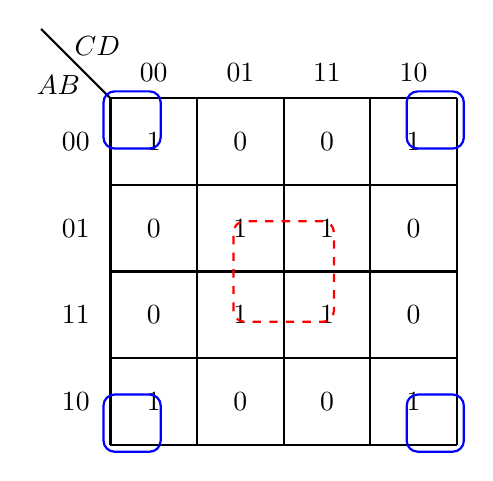
\begin{tikzpicture}[scale=1.1]
    \draw[thick] (0,0) grid (4,4);
    \draw[thick] (0,4) -- (-0.8,4.8);
    \node at (-0.6, 4.15) {$AB$};
    \node at (-0.15, 4.6) {$CD$};
    \node at (0.5, 4.3) {$00$}; \node at (1.5, 4.3) {$01$}; \node at (2.5, 4.3) {$11$}; \node at (3.5, 4.3) {$10$};
    \node at (-0.4, 3.5) {$00$}; \node at (-0.4, 2.5) {$01$}; \node at (-0.4, 1.5) {$11$}; \node at (-0.4, 0.5) {$10$};
    % Values
    \node at (0.5, 3.5) {1}; \node at (1.5, 3.5) {0}; \node at (2.5, 3.5) {0}; \node at (3.5, 3.5) {1};
    \node at (0.5, 2.5) {0}; \node at (1.5, 2.5) {1}; \node at (2.5, 2.5) {1}; \node at (3.5, 2.5) {0};
    \node at (0.5, 1.5) {0}; \node at (1.5, 1.5) {1}; \node at (2.5, 1.5) {1}; \node at (3.5, 1.5) {0};
    \node at (0.5, 0.5) {1}; \node at (1.5, 0.5) {0}; \node at (2.5, 0.5) {0}; \node at (3.5, 0.5) {1};
    % Group 1: corners
    \draw[thick, blue, rounded corners] (-0.08, 3.42) rectangle (0.58, 4.08);
    \draw[thick, blue, rounded corners] (3.42, 3.42) rectangle (4.08, 4.08);
    \draw[thick, blue, rounded corners] (-0.08, -0.08) rectangle (0.58, 0.58);
    \draw[thick, blue, rounded corners] (3.42, -0.08) rectangle (4.08, 0.58);
    % Group 2: center
    \draw[thick, red, rounded corners, dashed] (1.42, 1.42) rectangle (2.58, 2.58);
\end{tikzpicture}
\end{center}

\textbf{Langkah 2:} Identifikasi kelompok:
\begin{itemize}
    \item \textcolor{blue}{Kelompok 1}: 4 sel di empat sudut $\{m_0, m_2, m_8, m_{10}\}$ --- double wrap-around. $C = 0$ dan $D = 0$ konstan $\Rightarrow$ suku: $C'D'$
    \item \textcolor{red}{Kelompok 2}: 4 sel di tengah $\{m_5, m_7, m_{13}, m_{15}\}$ --- $C = 1$ dan $D = 1$ konstan $\Rightarrow$ suku: $CD$
\end{itemize}

\textbf{Hasil}: $F = C'D' + CD$

Perhatikan bahwa $C'D' + CD = C \odot D$ (XNOR), yaitu fungsi yang bernilai 1 ketika $C$ dan $D$ memiliki nilai yang sama. Ini menunjukkan bahwa K-Map tidak hanya menyederhanakan ekspresi, tetapi juga dapat mengungkap struktur logis yang tersembunyi.
\end{contoh}
